\documentclass{beamer}

\usetheme{metropolis}

\usepackage[ngerman]{babel}
\usepackage[autostyle=true,german=quotes]{csquotes}
\usepackage[linewidth=1pt]{mdframed}
\usepackage{hyperref}
\usepackage{makecell}
\usepackage{pifont}
\usepackage{tikz}
\usetikzlibrary{positioning, calc, arrows, fit, decorations.pathreplacing, shapes, shapes.multipart, snakes}
\usepackage{verbatim}
\usepackage{textcomp}
\usepackage{centernot}
\usepackage{tabularx}
\usepackage{ulem}
%\usepackage{pdfpages}

\batchmode

\hypersetup{
	colorlinks,
	urlcolor=blue,
	linkcolor=black % for ToC
}
\newenvironment{qaa}[1]{
	#1

	\begin{mdframed}
		\small
}{
	\end{mdframed}
}

\newcommand{\true}{\ding{51}}
\newcommand{\false}{\ding{55}}
\newcommand{\code}[1]{
	\begin{mdframed}
		\verbatiminput{#1}
	\end{mdframed}
}


\title{Tutorium 09: \texttt{let}-Polymorphismus}
% \subtitle{}
\author{David Kaufmann}
\institute{Tutorium Programmierparadigmen am KIT}
\date{09. Januar 2023}


\begin{document}

\begin{frame}
    \titlepage
\end{frame}

\section{Rückblick}

\begin{frame}{Rückblick}
    Bisherige Themen:

    \begin{itemize}
        \item Haskell: Funktionale Programmierung
        \item Lambda-Kalkül: Beta-Reduktion, Church-Encodings
        \item Typisierung: Lambda-Typen, Let, Typinferenz
        \item Prolog: Logische Programmierung
    \end{itemize}

    Ab jetzt:

    \begin{itemize}
        \item Parallelprogrammierung: MPI, Java
        \item Design by Contract: OpenJML
        \item Compiler: Parser + Java ByteCode
    \end{itemize}
\end{frame}

\section{ÜB 7/8}

\section{\textsc{Let}-Polymorphismus}

\begin{frame}{\textsc{Let}-Polymorphismus: Motivation}
  \begin{equation*}
    \lam{f}{\app{f}{f}}
  \end{equation*}

  \begin{itemize}
    \item Diese Funktion verwendet $f$ auf zwei Arten:
    \begin{itemize}
      \item $\alpha \to \alpha$: Rechte Seite.
      \item $(\alpha \to \alpha) \to (\alpha \to \alpha)$: Linke Seite, nimmt $f$ als Argument und gibt es zurück.
    \end{itemize}
    \pause
    \item Problem: $\alpha \to \alpha$ und $(\alpha \to \alpha) \to (\alpha \to \alpha)$ sind nicht unifizierbar!
    \begin{itemize}
      \item \enquote{occurs check}: $\alpha$ darf sich nicht selbst einsetzen.
    \end{itemize}
  \item Idee: Bei jeder Verwendung eines polymorphen Typen erzeugen wir \emph{neue Typvariablen}, um diese Beschränkung zu umgehen.
  \end{itemize}
\end{frame}

\begin{frame}{Typschemata und Instanziierung}
  \only<1>{
    \begin{itemize}
      \item Idee: Bei jeder Verwendung eines polymorphen Typen erzeugen wir \emph{neue Typvariablen}, um diese Beschränkung zu umgehen.
      \item Ein \emph{Typschema} ist ein Typ, in dem manche Typvariablen allquantifiziert sind:
    \end{itemize}

    \begin{align*}
      \phi     & = \forall \alpha_1 . \; ... \; \forall \alpha_n . \tau \\
      \alpha_i & \in FV(\tau)
    \end{align*}
  }

  \only<2>{
    \begin{itemize}
      \item Ein Typschema spannt eine Menge von Typen auf, mit denen es \emph{instanziiert} werden kann:
    \end{itemize}

    \begin{align*}
      \forall \alpha . \alpha \to \alpha & \succeq \text{int} \to \text{int} \\
      \forall \alpha . \alpha \to \alpha & \succeq \tau \to \tau \\
      \forall \alpha . \alpha \to \alpha & \not\succeq \tau \to \sigma \\
      \forall \alpha . \alpha \to \alpha & \not\succeq \tau \to \tau \to \tau \\
      \forall \alpha . \alpha \to \alpha & \succeq (\tau \to \tau) \to (\tau \to \tau)
    \end{align*}
  }
\end{frame}

\begin{frame}{Zusammenfassung}
    Def. aus VL: Für $n \in \mathbb{N}_0$ heist $\forall\alpha_1. \dots\forall\alpha_n. \tau$ \textbf{Typschema}. Es bindet freie Typvariablen $\alpha_1,\dots,\alpha_n$ in $\tau$.

    Def. aus VL: Für Typen $\tau_1, \dots, \tau_n$ ist der Typ $\tau[\alpha_1 \mapsto \tau_1, \dots, \alpha_n \mapsto \tau_n]$ eine \textbf{Instanziierung} vom Typschema $\forall\alpha_1. \dots\forall\alpha_n. \tau$. \\
    Schreibweise: $\forall\alpha_1. \dots\forall\alpha_n. \tau \succeq \tau[\alpha_1 \mapsto \tau_1, \dots, \alpha_n \mapsto \tau_n]$

    Das Typschema $ta(\tau,\Gamma) = \forall\alpha_1. \dots\forall\alpha_n. \tau$ heißt \textbf{Typabstraktion} von $\tau$ relativ zu $\Gamma$, wobei $\alpha_i \in \text{FV}(\tau) \setminus \text{FV}(\Gamma)$
\end{frame}

\begin{frame}{\textsc{Let}-Polymorphismus}
  \only<1>{
    Um Typschemata bei der Inferenz zu verwenden, müssen wir zunächst die Regel für Variablen anpassen:

    \begin{mathpar}
      \inferrule{
        \Gamma(x) = \phi \\
        \phi \succeq_{\text{frische $\alpha_i$}} \tau
      }{
        \Gamma \vdash x : \alpha_j
      } \textsc{Var} \\
      \text{Constraint:} \; \{ \alpha_j = \tau \}
    \end{mathpar}

    \begin{itemize}
      \item $\succeq_\text{frische $\alpha_i$}$ instanziiert ein Typschema mit $\alpha_i$, die noch nicht im Baum vorkommen.
      \item Jetzt brauchen wir noch eine Möglichkeit, Typschemata zu erzeugen.
    \end{itemize}
  }

  \only<2>{
    Mit einen \textsc{Let}-Term wird ein Typschema eingeführt:

    \begin{mathpar}
      \inferrule{
        \Gamma \vdash t_1 : \alpha_i \\
        \Gamma' \vdash t_2 : \alpha_j
      }{ 
        \Gamma \vdash \texttt{let} \;\; x = t_1 \;\; \texttt{in} \;\; t_2 : \alpha_k
      } \textsc{Let}
    \end{mathpar}

    \pause

    \begin{align*}
      \sigma_{let} &= mgu(C_{let}) \\
           \Gamma' &= \sigma_{let}(\Gamma), x : ta(\sigma_{let}(\alpha_i), \sigma_{let}(\Gamma)) \\
          C'_{let} &= \{ \alpha_n = \sigma_{let}(\alpha_n) \mid \sigma_{let}(\alpha_n) \;\; \text{ist definiert} \}
    \end{align*}

    Constraints: $C'_{let} \cup C_{body} \cup \{ a_j = a_k \}$
  }
\end{frame}

\begin{frame}{Übung}
    $$let \: f=\lambda x.2 \: in \: f(f \: true):\text{int}$$

    Gegeben:\\
    $\lambda x.2:\alpha \rightarrow \text{int}$ \\ 
    $\forall \alpha. \, \alpha \rightarrow \text{int} \succeq \text{bool} \rightarrow \text{int} \; \text{oder} \; \forall \alpha. \, \alpha \rightarrow \text{int} \succeq \text{int} \rightarrow \text{int}$

    \begin{figure}
        \centering
        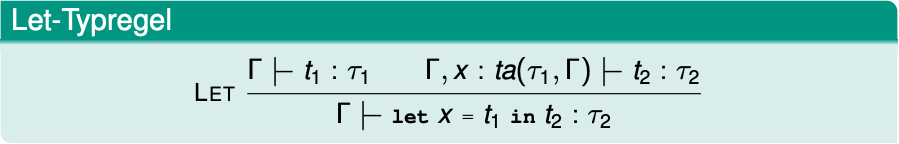
\includegraphics[width=0.9\textwidth]{slides/images/let_regel.png}
    \end{figure}

    \begin{figure}
        \centering
        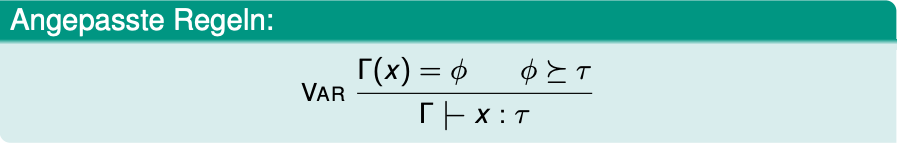
\includegraphics[width=0.9\textwidth]{slides/images/var_regel.png}
    \end{figure}
\end{frame}

\section{Herleitung}

\begin{frame}{Typinferenz ohne \texttt{let}}
    \begin{itemize}
        \item Herleitungsbaum aufstellen (mit den Regeln und frischen Variablen für Typen in den Voraussetzungen
        \item Sammle dabei Constraints, die erfüllt sein müssen damit der Herleitungsbaum gültig ist
        \item Bestimme mgu des Gleichungssystems (Robinson Algorithmus)
    \end{itemize}
\end{frame}

\begin{frame}{Typinferenz mit \texttt{let}-Regel}
    \begin{itemize}
        \item Betrachte zunächst nur den linken Teilbaum, um $\tau_1$ zu berechnen
            \begin{itemize}
                \item Constraints: $C_{\text{let}}$
                \item $\sigma_{\text{let}} = \text{mgu}(C_{\text{let}})$
            \end{itemize}
        \item Berechne $\Gamma':= \sigma_{\text{let}}(\Gamma), x: ta(\sigma_{\text{let}}(\tau_1), \sigma_{\text{let}}(\Gamma))$
        \item Benutze $\Gamma'$ im rechten Teilbaum, sammle Constrains in $C_{\text{body}}$
        \item Ergebnisconstraints sind $C_{\text{let}}' \cup C_{\text{body}} \cup$ mit $C_{\text{let}}' := \{\alpha_n = \sigma_{\text{let}}(\alpha_n)|\sigma_{\text{let}} \: \text{definiert für} \: \alpha_n\}$
    \end{itemize}
\end{frame}

\begin{frame}{Beispiel: \textsc{Let}-Polymorphismus}
    $$\vdash \texttt{let} \;\; f = \lam{x}{x} \;\; \texttt{in} \;\; \app{f}{f} : \alpha_1$$
\end{frame}

\begin{frame}{Beispiel: \textsc{Let}-Polymorphismus}
    \scriptsize
    \begin{mathpar}
      \inferrule{
        \inferrule{
          ...
        }{
          \vdash \lam{x}{x} : \alpha_2
        } \textsc{Abs} \\
        \inferrule{
          \inferrule{
            \Gamma'(f) = \forall \alpha_5 . \alpha_5 \to \alpha_5 \\\\
            \succeq \alpha_8 \to \alpha_8
          }{
            \Gamma' \vdash f : \alpha_6
          } \textsc{Var} \\
          \inferrule{
            \Gamma'(f) = \forall \alpha_5 . \alpha_5 \to \alpha_5 \\\\
            \succeq \alpha_9 \to \alpha_9
          }{
            \Gamma' \vdash f : \alpha_7
          } \textsc{Var}
        }{
          \Gamma' \vdash \app{f}{f} : \alpha_3
        } \textsc{App}
      }{ 
        \vdash \texttt{let} \;\; f = \lam{x}{x} \;\; \texttt{in} \;\; \app{f}{f} : \alpha_1
      } \textsc{Let}
    \end{mathpar}

    \begin{align*}
           C_{let} &= \{ \alpha_2 = \alpha_4 \to \alpha_5, \alpha_4 \to \alpha_5 \} \\
      \sigma_{let} &= \unifier{\su{\alpha_2}{\alpha_5 \to \alpha_5}, \su{\alpha_4}{\alpha_5}} \\
      \Gamma'      &= x : \forall \alpha_5 . \alpha_5 \to \alpha_5 \\
          C'_{let} &= \{ \alpha_2 = \alpha_5 \to \alpha_5, \alpha_4 = \alpha_5 \} \\
          C_{body} &= \{ \alpha_6 = \alpha_7 \to \alpha_3, \alpha_6 = \alpha_8 \to \alpha_8, \alpha_7 = \alpha_9 \to \alpha_9 \} \\
                 C &= C'_{let} \cup C_{body} \cup \{ \alpha_3 = \alpha_1 \}
    \end{align*}
\end{frame}

\section{Klausuraufgaben}
\end{document}